\documentclass[11pt]{article}
\usepackage{geometry}
\geometry{letterpaper, margin=1in}
\usepackage{graphicx}
\usepackage{amsmath}
\usepackage{amssymb}
\usepackage{listings}
\usepackage{color}
\usepackage{float}
\usepackage{hyperref}

\definecolor{codegreen}{rgb}{0,0.6,0}
\definecolor{codegray}{rgb}{0.5,0.5,0.5}
\definecolor{codepurple}{rgb}{0.58,0,0.82}
\definecolor{backcolour}{rgb}{0.95,0.95,0.92}

\lstdefinestyle{mystyle}{
    backgroundcolor=\color{backcolour},   
    commentstyle=\color{codegreen},
    keywordstyle=\color{magenta},
    numberstyle=\tiny\color{codegray},
    stringstyle=\color{codepurple},
    basicstyle=\ttfamily\footnotesize,
    breakatwhitespace=false,         
    breaklines=true,                 
    captionpos=b,                    
    keepspaces=true,                 
    numbers=left,                    
    numbersep=5pt,                  
    showspaces=false,                
    showstringspaces=false,
    showtabs=false,                  
    tabsize=2
}

\lstset{style=mystyle}

\title{CMS/CS/EE/IDS 144 HW 5: Centrality \& Games}
\author{Maurice Hanisch}
\date{February 17, 2026}

\begin{document}

\maketitle

\section{Discovering Clusters}

\subsection{Symmetric Stochastic Block Model (SSBM)}

In this part, we generated a SSBM network with $n=30$, $k=3$, $A=0.7$, and $B=0.1$. We compared $k$-means and spectral clustering algorithms using the implementation in Listing~\ref{lst:p1a}.

\begin{figure}[H]
    \centering
    
\includegraphics[width=0.7\linewidth]{figs/p1a_ground_truth.png}
    \caption{Ground Truth Clusters for SSBM}
    \label{fig:p1a_ground}
\end{figure}

\begin{figure}[H]
    \centering
    
\includegraphics[width=0.48\linewidth]{figs/p1a_kmeans.png}
    
\includegraphics[width=0.48\linewidth]{figs/p1a_spectral.png}
    \caption{Clustering Results for SSBM: K-Means (left) and Spectral Clustering (right)}
    \label{fig:p1a_results}
\end{figure}

\paragraph{Discussion:}
Both K-Means and Spectral Clustering recovered the ground truth clusters (Figure~\ref{fig:p1a_ground}) perfectly, as shown in Figure~\ref{fig:p1a_results} ($ARI = 1.000$). 

As highlighted in Note 1 of the assignment, the two algorithms interpret the data differently. For the SSBM graph, which is natively represented by its adjacency matrix:

\begin{itemize}
    \item \textbf{K-Means Interpretation:} We pass the adjacency matrix as input. K-Means interprets each row (or column) as a point in $n$-dimensional space. Each row acts as a "connectivity signature" or "neighborhood feature vector." Since nodes within the same community have a much higher probability of connecting to each other ($A=0.7$) than to others ($B=0.1$), their signatures will be geometrically close in $\mathbb{R}^n$. The Euclidean distance between rows effectively measures the similarity of their connection patterns, allowing K-Means to find the clusters.
    \item \textbf{Spectral Clustering Affinity:} Since we are already working with an adjacency matrix that defines the graph structure, we use \texttt{affinity='precomputed'}. This choice treats the adjacency matrix itself as the similarity matrix. This follows the conventional definition of spectral clustering on graphs, where the algorithm leverages the spectrum of the Laplacian derived from the connectivity to embed the nodes in a low-dimensional space before clustering.
\end{itemize}

The perfect recovery demonstrates that for this level of noise ($B=0.1$ vs $A=0.7$), both the direct neighborhood signatures and the spectral properties of the graph are highly discriminative.

\subsection{Circle Graph}

We generated a circle graph with $n=500$ and $\sigma=0.01$ using the code in Listing~\ref{lst:p1b}.

\begin{figure}[H]
    \centering
    
\includegraphics[width=0.7\linewidth]{figs/p1b_ground_truth.png}
    \caption{Ground Truth Clusters for Circle Graph}
    \label{fig:p1b_ground}
\end{figure}

\begin{figure}[H]
    \centering
    
\includegraphics[width=0.48\linewidth]{figs/p1b_kmeans.png}
    
\includegraphics[width=0.48\linewidth]{figs/p1b_spectral.png}
    \caption{Clustering Results for Circle Graph: K-Means (left) and Spectral Clustering (right)}
    \label{fig:p1b_results}
\end{figure}

\paragraph{Discussion:}
There is a stark difference between the two algorithms here (see Figure~\ref{fig:p1b_results}). K-Means ($ARI \approx 0$) fails completely because it assumes clusters are convex and separable by linear boundaries. Since one circle is nested inside the other (Figure~\ref{fig:p1b_ground}), no linear hyperplane can separate them.
Spectral Clustering ($ARI = 1.000$) handles this perfectly. Using the \texttt{nearest\_neighbors} affinity function (as implemented in Listing~\ref{lst:p1b}), it constructs a graph where edges only exist between nearby points. The inner and outer circles form two separate connected components, which the spectral embedding maps into highly separable regions in the eigen-space.

\section{Braess's Paradox Simulation}

\subsection{Initial Traffic Network (Part a)}

We simulated 4000 drivers on the $S \to A \to E$ and $S \to B \to E$ paths using the simulation engine in Listing~\ref{lst:braess_engine} and the runner in Listing~\ref{lst:p2}.

\begin{figure}[H]
    \centering
    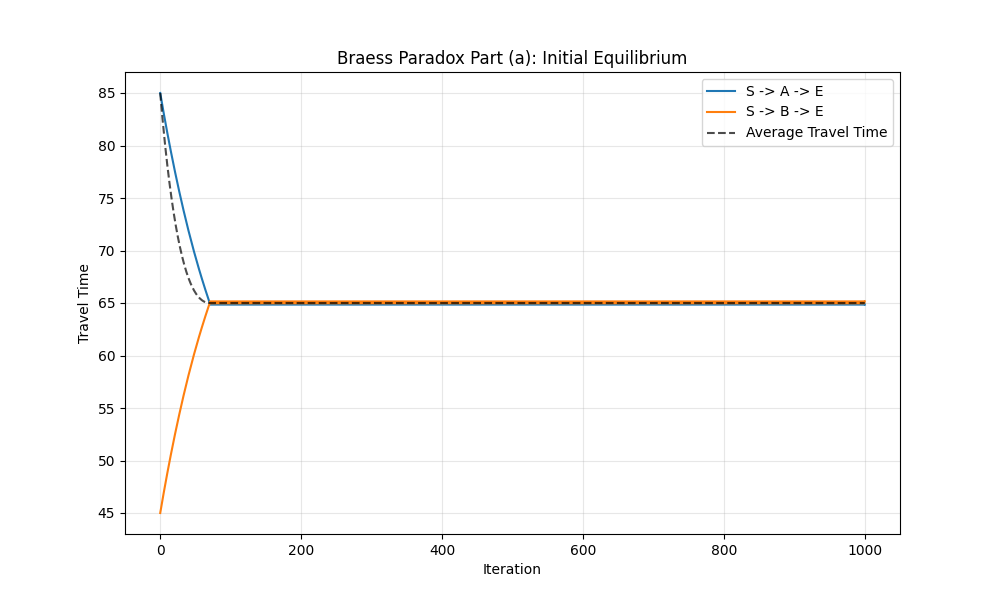
\includegraphics[width=0.8\linewidth]{figs/p2a_plot.png}
    \caption{Traffic equilibrium without the shortcut.}
    \label{fig:p2a}
\end{figure}

\paragraph{Results:}
As shown in Figure~\ref{fig:p2a}, the system reached equilibrium with approximately 2000 drivers on each path (Final distribution: Top = 2004, Bottom = 1996). 
The final travel times were: Path 1 $\approx 65.04$, Path 2 $\approx 64.96$. 
The average travel time was $65.00$. This is an equilibrium because the costs are nearly identical, and any driver switching paths would not significantly improve their time.

\subsection{Adding the Shortcut (Part b)}

We added the $A \to B$ edge with $T(x)=0$.

\begin{figure}[H]
    \centering
    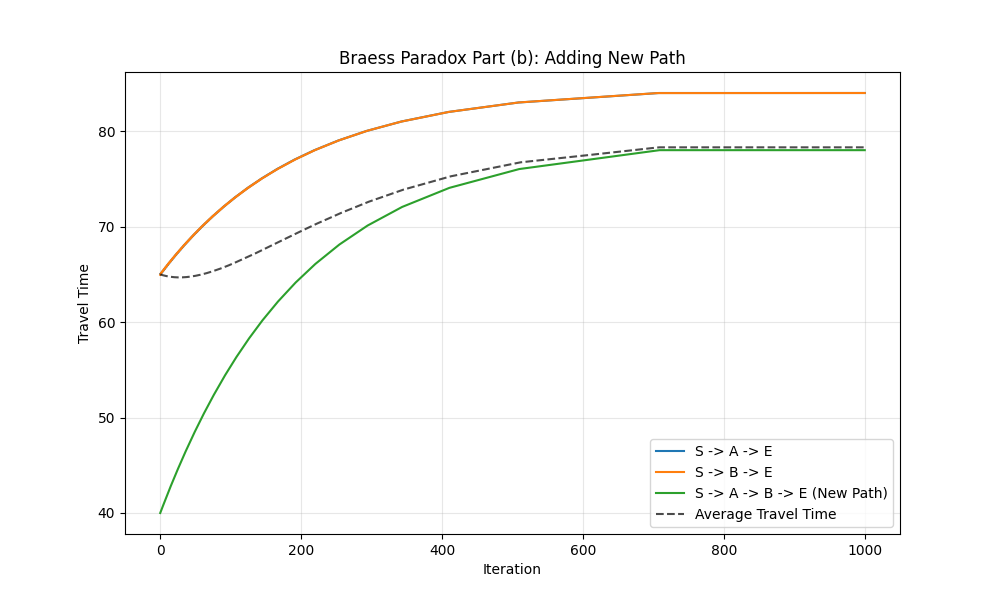
\includegraphics[width=0.8\linewidth]{figs/p2b_plot.png}
    \caption{Simulation of Braess's Paradox after adding $A \to B$.}
    \label{fig:p2b}
\end{figure}

\paragraph{Results:}
The simulation results in Figure~\ref{fig:p2b} show that the new distribution moved nearly all drivers to the middle path $S \to A \to B \to E$ (Final distribution: Top = 99, Bottom = 99, Middle = 3802).
The new average travel time is approximately $78.32$. 
Compared to the initial $65.00$ in Figure~\ref{fig:p2a}, the travel time \textbf{increased} significantly. This confirms Braess's Paradox: adding capacity (a free shortcut) worsened the global outcome. 

This is still an equilibrium. At the final state:
\begin{itemize}
    \item Middle path cost: $(3802+99)/100 + 0 + (3802+99)/100 = 78.02$.
    \item Top path cost: $(3802+99)/100 + 45 = 84.01$.
    \item Bottom path cost: $45 + (3802+99)/100 = 84.01$.
\end{itemize}
Individual drivers have no incentive to switch back to the original paths because $78.02 < 84.01$.

\subsection{Intuitive Explanation (Part c)}

Drivers flock to the new path because, from an individual's perspective, the $S \to A \to B \to E$ path is always better or equal to the alternatives for a given distribution of others. Specifically, for any flow $x_{SA}$ and $x_{BE}$, the path $S \to A \to B \to E$ has cost $x_{SA}/100 + x_{BE}/100$, while $S \to A \to E$ has $x_{SA}/100 + 45$. Since $x_{BE}/100$ can't exceed $40$, the middle path looks cheaper than the top one. 
However, when everyone chooses this "shortcut", the congestion on the shared segments ($S \to A$ and $B \to E$) increases so much that the total time exceeds the original state. They don't switch back because even in the congested state, the shortcut is still faster than the alternatives \textit{given the current congestion}. This is a classic example of a Nash Equilibrium that is not socially optimal.

\section{Routing Games with Tolls}

\textbf{Problem 5:} Prove that any optimal strategy for our original game is a Nash equilibrium for this new game (with link cost functions $c^*_e(\cdot)$).

\textbf{Solution:}

In an atomic routing game where each user has traffic $r_i = 1$, we can analyze the behavior of selfish players by constructing a potential function. A game with edge cost functions $\tilde{c}_e(x)$ is an exact potential game with Rosenthal's potential function:
$$ \Phi(f) = \sum_{e \in E} \sum_{k=1}^{f_e} \tilde{c}_e(k) $$
where $f_e$ is the number of players using edge $e$. By the properties of exact potential games, any flow profile $f$ that minimizes the potential function $\Phi(f)$ is a pure-strategy Nash Equilibrium.

For the new game, the cost functions are given by marginal cost pricing:
$$ c^*_e(x) = c_e(x) + (x-1)\left(c_e(x) - c_e(x-1)\right) $$

We can rewrite the expression for $c^*_e(x)$ as follows:
$$ c^*_e(x) = x c_e(x) - (x-1)c_e(x-1) $$

Now, let's construct the potential function $\Phi_{new}(f)$ for this new game by substituting $c^*_e(x)$ into Rosenthal's potential function formula:
$$ \Phi_{new}(f) = \sum_{e \in E} \sum_{k=1}^{f_e} c^*_e(k) $$
$$ \Phi_{new}(f) = \sum_{e \in E} \sum_{k=1}^{f_e} \left[ k c_e(k) - (k-1)c_e(k-1) \right] $$

Observe that the inner sum over $k$ is a telescoping sum. Let $S_k = k c_e(k)$. The term inside the sum is exactly $S_k - S_{k-1}$. Expanding the sum for a given edge $e$, we get:
$$ \sum_{k=1}^{f_e} \left[ k c_e(k) - (k-1)c_e(k-1) \right] = (1 \cdot c_e(1) - 0) + (2 \cdot c_e(2) - 1 \cdot c_e(1)) + \dots + (f_e c_e(f_e) - (f_e-1)c_e(f_e-1)) $$
All intermediate terms cancel out, leaving only the final term:
$$ \sum_{k=1}^{f_e} c^*_e(k) = f_e c_e(f_e) $$

Substituting this back into the potential function gives:
$$ \Phi_{new}(f) = \sum_{e \in E} f_e c_e(f_e) $$

Notice that $\Phi_{new}(f)$ is exactly the objective function (social cost) $C(f)$ of the \textit{original} game!
$$ \Phi_{new}(f) = C(f) = \sum_{e \in E} f_e c_e(f_e) $$

Let $f^*$ be an optimal strategy (flow profile) for the original game. By definition, $f^*$ minimizes the social cost $C(f)$. Therefore, $f^*$ must also minimize the potential function $\Phi_{new}(f)$ of the new game. 

Since $f^*$ is a global minimum of the exact potential function $\Phi_{new}(f)$, no player can unilaterally deviate to lower their personal cost (as any such deviation would strictly decrease the potential, which is impossible at a global minimum). Thus, $f^*$ is a Nash equilibrium for the new game.

\newpage
\appendix
\section{Code Listings}

\subsection{Clustering Utilities}
The utilities for generating SSBM and visualizing graphs are provided in Listing~\ref{lst:utils}.
\lstinputlisting[language=Python, caption=clustering\_utils.py, label=lst:utils]{../code/clustering_utils.py}

\subsection{Problem 1a Solver}
The experimental setup for SSBM clustering is shown in Listing~\ref{lst:p1a}.
\lstinputlisting[language=Python, caption=solve\_p1a.py, label=lst:p1a]{../code/solve_p1a.py}

\subsection{Problem 1b Solver}
The experimental setup for Circle graph clustering is shown in Listing~\ref{lst:p1b}.
\lstinputlisting[language=Python, caption=solve\_p1b.py, label=lst:p1b]{../code/solve_p1b.py}

\subsection{Braess Simulation Engine}
The core simulation logic for Braess's Paradox is implemented in Listing~\ref{lst:braess_engine}.
\lstinputlisting[language=Python, caption=braess\_simulation.py, label=lst:braess_engine]{../code/braess_simulation.py}

\subsection{Problem 2 Solver}
The script used to run the traffic simulations is shown in Listing~\ref{lst:p2}.
\lstinputlisting[language=Python, caption=solve\_p2.py, label=lst:p2]{../code/solve_p2.py}

\end{document}
